\section{Force \& Motion}

\subsection{force \& motion: an introduction}

in physics, a force appears when two bodies interact with one another

\cmt you will encounter various types of forces in this course, some of which are

\begin{compactitem}
	\item[--] \emph{weight}: the gravitational attraction acting on any object exerted by the earth
	
	\item[--] \emph{tension}: a force in a string, a rope, a chain, etc. when it is being pulled
	
	\item[--] \emph{normal contact}: when a body's surface is compressed, there reacts a normal contact force\footnote{Examples of normal contact force are support force that stops a desk from sinking into the ground, and the impact on a football when you kick it, etc.}
	
	\item[--] \emph{friction}: a force that resists relative motion when two surfaces tend to slide over one another
	
	\item[--] \emph{resistance}: also called drag force, this is experienced when a body travels through a medium

	
	\item[--] \emph{upthrust}: an upward force acting on an object immersed in a fluid
	
	\item[--] \emph{electric force}: an attractive or repulsive interaction between electrically charged objects
	
%	\item[--] \emph{magnetic force}: an attractive or repulsive interaction between magnets or electric currents
\end{compactitem}

detailed features of these forces follow later in the notes.

\cmt a force can produce various effects to the object, the effect could be

\begin{compactitem}
	\item[--] an increase/decrease in speed
	
	\item[--] a change in the direction of motion
	
	\item[--] causing the object to rotate
	
	\item[--] a change in shape of the object
\end{compactitem}

in this and the next few chapters, we will be looking into each of these aspects

\cmt when more than one force act on a body, it is useful to find their \emph{resultant}, or the \emph{net force}

\begin{ilight}
	\keypoint{resultant force}, or \keypoint{net force}, is a single force that has the same effect as all forces acting on an object combined
\end{ilight}

\emph{vector sum} of all of the individual forces gives the resultant force

\cmt in this chapter, we will study the dynamics of \emph{point masses}

\keypoint{point mass} is an idealization that the object has a mass but does not take up any space

position of an object treated as a point mass is specified with a geometric point in space

this is a simplification when size, shape, rotation, or structure of object are not important




\subsection{Newton's laws of motion}\index{Newton's laws of motion}

Newton's laws of motion\footnote{These three laws were first addressed by \emph{Isaac Newton} in his famous work \emph{Mathematical Principles of Natural Philosophy}, or simply the \emph{Principia}. The three-volume work was first published in 1687, and was soon recognised as one of the most important works in the history of science. Apart the from the three laws that laid the foundations for classical mechanics, the \emph{Principia} also stated \emph{the law of gravitation}, and accounted for planetary orbits and tides and other phenomena.} are three laws that form the basis of classical mechanics

they describe the relationships between motion of an object and forces acting on it


\subsubsection{first law}

\begin{ilight}
	\keypoint{Newton's first law} states that an object continues in its state of rest or uniform motion at constant velocity if there is no resultant force acting
\end{ilight}


\cmt any object `dislikes' any change to its state of motion, uniform motion tends to persist forever

this tendency to resist changes in motion is called the \keypoint{inertia}

Newton's first law is also called \emph{the law of inertia}

\cmt if there is no change in state of motion, the object is said to be in \keypoint{equilibrium}\index{equilibrium}

equilibrium could be either \emph{static} (being at rest) or \emph{dynamic} (steadily moving in a straight line)

both cases require zero resultant force

\cmt Newton’s law of inertia is placed to establish frames of reference

it is in an reference frame that notions of displacement, velocity and acceleration can be defined

an \keypoint{inertial reference frame} is one in which Newton’s laws hold
\footnote{Inertial frame is not unique. An observer moving at constant velocity to an inertial observer is in a different inertial frame, since constant velocity of object added to a constant relative velocity is still a constant velocity. Two inertial observers would disagree on a body's velocity, but they would agree that the body maintains its velocity in absence of net force, i.e., they will observe the same physics phenomena. This is known as the \emph{equivalence principle}.}

%\begin{example}{Suspension of a slinky}
%	If a slinky is freely suspended, one notices that the degree to which the slinky is stretched increases uniformly with height.
%	
%	Since the slinky is in a state of rest, all net force is cancelled throughout the entire slinky, i.e., the tension at any point balances the weight of the slinky beneath it. So the higher it goes, the more weight is supported, so the top bit has to be stretched more to provide a greater tension to hold the bottom part.
%\end{example}


\subsubsection{second law}

if resultant force is non-zero, velocity of the object will change, i.e., force produces acceleration


\begin{ilight}
	\keypoint{Newton's second law} states that the acceleration is proportional to the resultant force and inversely proportional to the mass of the object
\end{ilight}

\cmt symbolically, we write $a \propto \frac{\fnet}{m}$

with consistent units of measure, this proportionality can be written as an exact equation:
\begin{equation}
a=\frac{\fnet}{m} \quad \text{or} \quad \boxed{\fnet=ma}
\end{equation}

\cmt SI unit of measurement for force $F$ is \keypoint{newton} (N)

a force of one newton acting a body of 1 kg produces an acceleration of 1 $\mpss$

\cmt note that the force in the equation $F=ma$ is the resultant force

to determine change in motion for a body, you should always ask what the resultant force is

\cmt acceleration produced is always in same direction of the net force

\cmt for same force, an object of greater mass has a smaller acceleration

hence mass is a measure of the \emph{inertia} of this object in response to a net force\index{inertia}

a definition for mass of an object from the point of view of Newton's laws can be stated as\footnote{The concept of mass can be defined in many different ways. You might be familiar with the definition for mass as the amount of matter an object possesses. I personally think this definition is a bit vague and does not tell you anything new. Thinking of mass as a measure of inertia surely brings more insights. Mass also tells the strength at which an object interacts with other bodies through the gravitational attraction. As you will see later, from the view of Albert Einstein, it is also possible to think of mass as a form of energy, which is my favourite definition for mass.}:

\begin{ilight}
	\keypoint{mass} is an intrinsic property of a body to resist any change in its state of motion
\end{ilight}

\example{A box of 6.0 kg is being pushed along a horizontal surface with a force of 30 N. The resistive force acting is 21 N. What is the acceleration of the box?}

\solc\begin{equation*}
	\fnet = F - f = ma \RA a = \frac{F-f}{m} = \frac{30-21}{6.0} = 1.5 \mpss \teoe
\end{equation*}

\example{A car of mass 800 kg is travelling at a speed of $20 \mps$. The driver then operates the brake pedal so a braking force of 2000 N gradually brings the car to stop. (a) What is the deceleration for the car? (b) What is the stopping distance?}

\sol using Newton's second law and noticing braking force acts opposite to direction of motion:

{
	\centering
	
	$\fnet = ma \RA -2000 = 800 \times a \RA a = -2.5 \mpss$
	
	$2as = v^2 - u^2 \RA s = \frac{v^2-u^2}{2a} = \frac{0^2 - 20^2}{2\times(-2.5)} = 80\text{ m}$
	
}

\feoe



	\begin{wrapfigure}{R}{0.2\textwidth}
		\vspace{-18pt}
		\begin{center}
			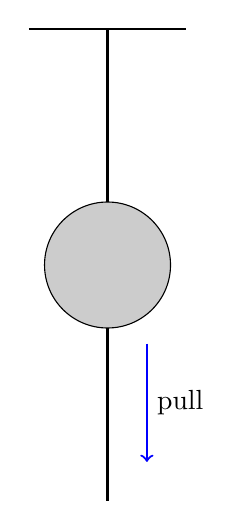
\begin{tikzpicture}[scale=1]
			\draw[thick] (-1,6) -- (1,6);
			\draw[thick] (0,6) -- (0,0);
			\draw[thick, ->, blue] (.5,2) -- (.5,0.5) node[midway, right]{\textcolor{black}{pull}};
			\draw[fill=gray!40] (0,3) circle[radius=.8];
			\end{tikzpicture}
		\end{center}
		\vspace{-20pt}
	\end{wrapfigure}
	
\example{A massive ball is suspended on a string. A second string is attached to the bottom of the ball. If one pulls the bottom string with a gradually increasing force, does the top string or the bottom string break first? What if the bottom string is jerked, which string breaks?}	
	
\sol when tension gradually increases, system is always in equilibrium

tensions in strings must have $T_\text{top} = T_\text{bottom} + mg$

top string suffers a greater force, so it breaks first
	
however, when bottom string is jerked, the ball tends to remain at rest due to its large mass, preventing sudden change to the tension in top string

so in this case bottom string is more likely to snap \eoe

%\begin{example}{Leviation of a slinky}
%	When the top end of the slinky is dropped, the information of the tension change must propagate to the bottom end before both sides begin to fall; the top of an extended slinky will drop while the bottom initially remains in its original position, compressing the spring.
%\end{example}




\subsubsection{third law}

every force is part of a pair of interactions between one body and another

when one body exerts a force on another, the second body also exerts a reaction on the first

\begin{ilight}
	\keypoint{Newton's third law}, also called the \keypoint{action-reaction principle}, states that action and reaction are always equal in magnitude, opposite in directions and of the same type
\end{ilight}

\example{Suggest the action and reaction force in the following cases: (a) A man stands on a bathroom scale. (b) A helicopter hovers in air. (c) The earth orbits around the sun.}

\sol (a) man exerts downward force on scale, scale exerts an upward reaction on man

(b) rotors of helicopter push air downwards, air exerts an upward force on helicopter

(c) sun pulls the earth through gravitational attraction, earth also attracts the sun in return \eoe


\subsubsection{force analysis \& free-body diagrams}

when doing mechanics problems, it is necessary to find all forces applied upon an object

to visualise all these forces, it is helpful to draw a \keypoint{free-body diagram} (FBD)\index{free-body diagram}

an FBD shows a simplified version of the body with arrows indicating forces applied

\newpage

it is recommended to follow the routine stated below when solving a mechanics problem

\begin{compactitem}
	\item[(1)] draw a FBD for the object in the problem
	
	\item[(2)] resolve and find the resultant force with aid of the FBD
	
	\item[(3)] apply Newton's laws to write down the equation of motion for the object
	
	\item[(4)] solve the equation(s) to find acceleration
	
	\item[(5)] use kinematic relations to deduce information about motion of the object
\end{compactitem}


% % % % % % % % % % % % % % % % % % % %

\subsection{types of forces}

\subsubsection{weight}\label{ch_weight}

all objects exert attractive forces of gravity upon each other\footnote{You will learn more about gravitational forces at A2 Level.}

\keypoint{weight} of a body is due to the gravitational pull from our planet -- the earth\index{weight}

weight $W$ of any object is proportional to its mass $m$: $\boxed{W=mg}$

$g$ is called the gravitational field strength, or the gravitational acceleration constant

\cmt at vicinity of earth's surface, gravitational field is almost uniform: $g \approx 9.81 \text{ N kg}^{-1}$

but this value for $g$ does not hold in a satellite orbit, on Mars, near a black hole, etc.

\cmt the concept of weight is different from mass in many aspects

\begin{compactitem}
	\item[--] weight is a force, so it is a vector (always acting downwards still makes a direction)
	
	mass is a scalar, it has magnitude only
	
	\item[--] weight is measured in newtons, mass is measured in kilograms
	
	\item[--] weight of object depends on its mass but also strength of gravitational field
	
	mass is an intrinsic property of object, so does not depend on force fields
	
	same object can have different weights on different planets, but its mass will be the same\footnote{Here we do not take into account the effects of \emph{relativity}. A clever student who has learned Einstein's theories might suggest the mass of the same object increases with its velocity.}
\end{compactitem}

\example{An astronaut finds that he weighs 300 N on the surface of Mars, where the gravitational field strength is known to be $3.7 \text{ N kg}^{-1}$. Find his mass and hence estimate his weight if he returns to his home on the Earth.}

\sol mass of astronaut: $m = \frac{W_M}{g_M} = \frac{300}{3.7} \approx 81.1 \text{ kg}$

weight on earth: $W_E = mg_E = 81.1 \times 9.81 \approx 795 \text{ N}$ \eoe

\subsubsection*{free fall}

all things on the earth fall because of the force of gravity

if we ignore the restraints such as air resistance and upthrust force on a falling object, say the object is under the influence of gravity only, then the object is in a state called \keypoint{free fall}



assuming the object is subject to gravity only, the resultant force is simply its weight

applying the Newton's second law, we have: $\fnet = W \RA ma = mg$

so acceleration of the freely-falling object is: $\boxed{a=g}$\footnote{In the derivation, the mass terms cancel out. Rigorously speaking, these are two different masses. One is the measure of inertia, and the other is a measure of gravitational force. It is experimentally found that the inertia mass and the gravitational mass are equal. The fact that the two masses are equal has profound reasons. We have shown here acceleration of free fall equals gravitational field strength, but Albert Einstein’s suggests that it is actually impossible to distinguish between a uniform acceleration and a uniform gravitational field. This idea lies at the heart of his \emph{general theory of relativity}. Those who are interested in this topic are recommended to start from here and do some online researches.}

\cmt this shows \keypoint{acceleration due to free fall} is simply equal to field strength $g$

so any object, regardless of its mass, has same acceleration due to free fall\footnote{In \S\ref{ch_freefall} and \S\ref{ch:projectile}, the statement that acceleration of free fall is constant in absence of air resistance was asserted without further explanation. Now you know why.}


\subsubsection{drag}

when a body moves through air, water or any fluid, it experiences resistance called drag force\index{drag}

\cmt factors that determine the value of fluid drag include

\titem relative speed of the object to the fluid ($v\up \ra f\up$)

\titem cross section of the object ($A\up \ra f\up$)

\titem shape of the object (streamlined shape has smaller drag)

\titem density of the fluid ($\rho\up \ra f\up$)

but what determines the drag force is a complicated issue\footnote{There are a few empirical formula for drag force, each of which is accurate under certain conditions.
	
	For an object moving through a fluid at low speeds (\emph{laminar flow}, no turbulence occurs), the resistance it experiences is proportional to its speed: $f=bv$, where $b$ is some constant which depends on fluid viscosity and the effective cross-sectional area of the object.
	
	If objects are moving at relative high speeds through the fluid such that \emph{turbulence} is produced behind the object, drag force is proportional to the speed squared: $ f = \frac{1}{2} \rho C_D A v^2$, where $\rho$ is the fluid's density, $A$ is the cross-sectional area, $C_D$ is a dimensionless quantity called the drag coefficient.}

\cmt drag force always acts in a direction to oppose relative motion of object through fluid




\subsubsection*{free fall through air}

\begin{wrapfigure}{r}{0.15\textwidth}
	\vspace*{-16pt}
	\centering
	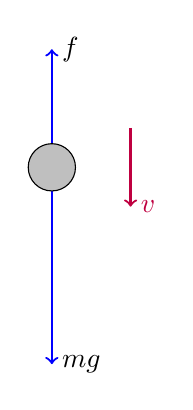
\begin{tikzpicture}
	\draw[thick,blue,->] (0,0) -- (0,-2.5) node[right,black]{$mg$};
	\draw[thick,blue,->] (0,0) -- (0,1.5) node[right,black]{$f$};
	\draw[fill=gray!50] (0,0) circle (0.3);
	\draw[thick,purple,->] (1,0.5) -- (1,-0.5) node[right]{$v$};
	\end{tikzpicture}
	\vspace*{-16pt}
\end{wrapfigure}

let's consider an object falling through air from a very high tower

forces acting are weight and air resistance (shown in the free-body diagram)

equation of motion for this falling object is:

{
	\centering
	
	$ \fnet = mg - f = ma $
	
}

as $v$ increases, air resistance $f$ increases, so net force $\fnet$ decreases

this means acceleration $a$ would decrease as object falls

i.e., speed will increase at a decreasing rate during the fall
\footnote{The velocity-time relation can be obtained for some simple models. Suppose air resistance is proportional to speed of the falling body, i.e., $f=bv$, then the equation of motion reads: $\fnet = m \frac{\dd v}{\dd t} = mg - bv$, where acceleration is written explicitly as the rate of change in velocity. With the initial conditions $v=0$ at $t=0$, we can solve this differential equation to obtain the speed of this falling object at any given time $t$:
\begin{equation*}
	\dd t = \frac{\dd v}{g - \frac{b}{m}v} \RA \int_0^t \dd t = \int_0^v \frac{\dd v}{g - \frac{b}{m}v} \RA t = -\frac{m}{b} \ln \left(g - \frac{b}{m}v \right) \Bigg|_0^v = -\frac{m}{b} \ln \left( 1 - \frac{bv}{mg}\right)
\end{equation*}
	
Rearrange the terms, we find: $v(t) = \frac{mg}{b} \left(1 - \ee^{-\frac{bt}{m}} \right) $}

%$v$-$t$ graph for this process is shown on the next page


\begin{figure}[ht]
	\centering
	\begin{tikzpicture}[xscale = 1.6,yscale=1.65]
	\draw [thick, <->] (7.5,0) node[below]{$t$} -- (0,0) --(0,3.6) node[left]{$v$};
	\draw [thick,blue,domain=0:7,samples=20,smooth,variable=\x] plot (\x,{2.5*(1-exp(-0.8*\x))});
	\draw [thick,orange] (0,0) -- (1.8,3.6);
	\draw [thick,dashed] (0,2.5) node[left]{$v_t$} -- (7,2.5);
	\draw [->] (3,0.6) node[note]{When air drag is small at low speed,\\ acceleration $a$ is slightly less than $g$.} -- (0.45,0.6);
	\draw [->] (5,1.6) node[note]{Gravity is offset by the increasing air drag, \\ the velocity tends to a terminal value $v_t$.} -- (5,2.4);
	\draw [->] (4.2,3.1) node[note]{In absense of air, an object falls freely \\ with constant acceleration $g\approx9.81\mpss$.} -- (1.6,3.1);
	\end{tikzpicture}
	\caption*{variation of velocity for a falling object through air}
\end{figure}

\cmt after sufficient long time, acceleration gradually decreases to zero

velocity gradually increases and tends to a maximum value

at this stage, equilibrium is restored: $f=mg$, object no longer accelerates

this constant final velocity is known as the \keypoint{terminal velocity}\index{terminal velocity}

\cmt at low speeds, air resistance is negligible, so $\fnet =ma \approx mg$

acceleration of object at start of the fall is similar to $g$

but as $v$ increases, acceleration decreases so $a$ becomes less than $g$




\example{An object of 5.0 kg falls through the atmosphere from a very high altitude. After some time, it falls at a constant speed of $70 \mps$. Assume there is no significant change in gravitational field during the fall and the air resistance is proportional to speed: $f=bv$. (a) Find the value of the coefficient $k$. (b) Find the acceleration of the object when it is falling at $30\mps$.}

\sol equilibrium between weight and air drag when falling at terminal speed, so
\begin{equation*}
	mg = bv_t \RA b = \frac{mg}{v_t} = \frac{5.0\times9.81}{70} \approx 0.70 \text{ kg s}^{-1}
\end{equation*}

at any instant, equation of motion is: $\fnet = ma = mg - bv$

at $30\mps$, acceleration is: $a = \frac{mg-bv}{m} = \frac{5.0\times9.81-0.70\times30}{5.0} \approx 5.6 \mpss$ \eoe

\subsubsection*{bubble rising in a liquid}

\begin{wrapfigure}{r}{0.15\textwidth}
	\vspace*{-16pt}
	\centering
	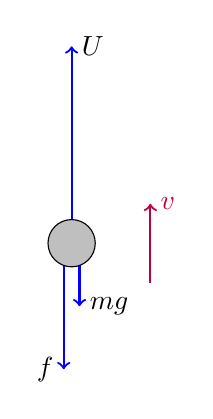
\begin{tikzpicture}
	\draw[thick,blue,->] (0.1,0) -- (0.1,-0.8) node[right,black]{$mg$};
	\draw[thick,blue,->] (-0.1,0) -- (-0.1,-1.6) node[left,black]{$f$};
	\draw[thick,blue,->] (0,0) -- (0,2.5) node[right,black]{$U$};
	\draw[fill=gray!50] (0,0) circle (0.3);
	\draw[thick,purple,->] (1,-0.5) -- (1,0.5) node[right]{$v$};
	\end{tikzpicture}
	\vspace*{-16pt}
\end{wrapfigure}

let's now consider bubbles formed at the bottom of a soda water

forces acting on bubble are weight, water resistance and upthrust

equation of motion for the rising bubble is:

{
	\centering
	
	$ \fnet = U - mg - f = ma $
	
}

as bubble moves faster, $f$ increases, then $\fnet$ decreases

so acceleration $a$ would gradually decrease to zero as bubble rises

speed of bubble increases and reaches a maximum value

at terminal speed, $a\to0$, one has: $U=f+mg$



\subsubsection{normal contact}

when two objects are in contact, the interaction between them is called the \emph{contact force}

\keypoint{normal contact force} is the component of contact force that is perpendicular to contact surface

\cmt by definition, normal contact is always at right angle to surface of contact

\cmt origin of normal contact is the \emph{electrostatic interaction} between atoms

when two objects are pressed against each other, surface atoms get close

\begin{wrapfigure}{r}{0.3\textwidth}
	\vspace*{-10pt}
	\centering
	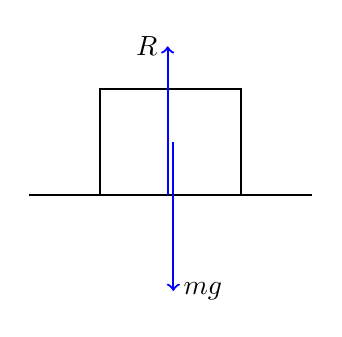
\begin{tikzpicture}[scale=0.9]
	\draw[thick] (-2,0) -- (2,0);
	\draw[thick] (-1,0) rectangle (1,1.5);
	\draw[thick,blue,->] (0.04,0.75) --++ (0,-2.1) node[right,black]{$mg$};
	\draw[thick,blue,->] (-0.04,0) --++ (0,2.1) node[left,black]{$R$};
	\end{tikzpicture}
	\vspace*{-5pt}
\end{wrapfigure}

electrostatic repulsion between electron clouds of the atoms prevent them from penetrating through one another


\example{A box of mass $m=4.0 \text{ kg}$ is resting on a horizontal ground. What is the normal contact force acting?}

\sol equilibrium between weight and normal contact, so
\begin{equation*}
	R-W=0 \RA R=mg = 4.0 \times9.81 \approx 39.2 \text{ N} \teoe
\end{equation*}

\begin{wrapfigure}{r}{0.24\textwidth}
	\vspace*{-10pt}
	\centering
	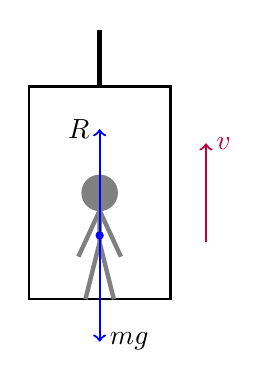
\begin{tikzpicture}[scale=0.9]
	\draw[thick] (-1,0) rectangle (1,3);
	\draw[fill, gray] (0,1.5) circle(0.25);
	\draw[ultra thick, gray] (0,1.5) -- (0,0.8) -- (-0.2,0) (0,0.8) -- (0.2,0);
	\draw[ultra thick, gray] (0,1.25) -- (-0.3,0.6) (0,1.25) -- (0.3,0.6);
	\draw[blue,fill] (0,.9) circle(0.05);
	\draw[thick,blue,->] (0,.9) --++ (0,-1.5) node[right,black]{$mg$};
	\draw[thick,blue,->] (0,.9) --++ (0,1.5) node[left,black]{$R$};
	\draw[ultra thick] (0,3) --++ (0,0.8);
	\draw[purple,thick,->] (1.5,0.8) --++ (0,1.4) node[right]{$v$};
	\end{tikzpicture}
	\vspace*{-5pt}
\end{wrapfigure}

\example{A man of $80$ kg stands in a lift. Find his apparent weight, i.e., the contact force, when the lift is (a) moving upwards at steady speed of $2.0 \mps$, (b) accelerating upwards at $2.0 \mpss$, (c) moving upwards but slowing down at a deceleration of $1.5 \mpss$.}

\sol forces acting on man are weight and normal contact

for either case, equation of motion for the man reads:

{

\centering

$\fnet = ma = R - mg$

}

so normal contact force: $R = mg + ma$

when rising at steady speed, man is in equilibrium ($a=0$), so: $R=mg = 80\times9.81 \approx 785 \text{ N}$

when accelerating upwards ($a = +2.0 \mpss$): $R = 80 \times 9.81 + 80 \times 2.0 \approx 945 \text{ N}$

when decelerating upwards ($a = -1.5 \mpss$): $R = 80 \times 9.81 + 80 \times (-1.5) \approx 665 \text{ N}$ \eoe


\example{A sleigh of mass 15 kg lies at rest on an icy ground. The surface is frictionless. A force $P$ of 75 N is applied to the sleigh. Find the normal contact force and the acceleration of the sleigh if $P$ is acting (a) horizontally, (b) at an angle $\alpha$ to the horizontal where $\tan\alpha=\frac{3}{4}$.}

\begin{wrapfigure}{r}{0.4\textwidth}
	\vspace*{-20pt}
	\centering
	\begin{minipage}[b]{0.2\textwidth}
		\centering
		\begin{tikzpicture}[scale=0.84]
		\draw[thick,fill] (0,0) circle(0.05);
		\draw[blue,thick,->] (0,0) -- (0,-3) node[right]{$mg$};
		\draw[blue,thick,->] (0,0) -- (0,3) node[right]{$R$};
		\draw[blue,thick,->] (0,0) -- (1.5,0) node[right]{$P$};
		\node at (0,-4) {(a)};
		\end{tikzpicture}
	\end{minipage}\hfil
	\begin{minipage}[b]{0.2\textwidth}
		\centering
		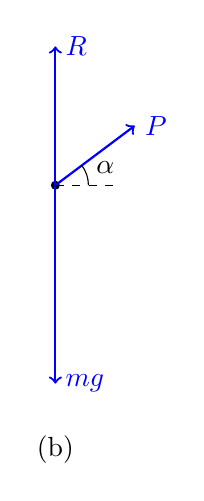
\begin{tikzpicture}[scale=0.84]
		\draw[thick,fill] (0,0) circle(0.05);
		\draw[blue,thick,->] (0,0) -- (0,-3) node[right]{$mg$};
		\draw[blue,thick,->] (0,0) -- (0,2.1) node[right]{$R$};
		\draw[blue,thick,->] (0,0) -- (1.2,0.9) node[right]{$P$};
		\draw[dashed] (0,0) -- (1,0);
		\draw(0.5,0) arc(0:36.89:0.5);
		\node at (19:0.8) {$\alpha$};
		\node at (0,-4) {(b)};
		\end{tikzpicture}
	\end{minipage}
\end{wrapfigure}

\sol free-body diagrams for both cases are shown

for both cases, no net force acts in vertical direction

net force in horizontal direction provides acceleration

when $P$ acts horizontally:

{
	\centering
	
	$ R = mg = 15\times 9.81 \approx 147 \text{ N}$
	
	$ P = ma \RA a = \frac{P}{m} = \frac{75}{15} = 5.0 \mpss $
		
}

when $P$ acts at angle $\alpha$:

{
	\centering
	
	$R + P\sin\alpha = mg \RA R = 15\times9.81-75\times\frac{4}{5} \approx 87 \text{ N}$
	
	\eqyskip $ P\cos\alpha = ma \RA a = \frac{P\cos\alpha}{m} = \frac{75\times\frac{3}{5}}{15} = 3.0 \mpss $
	
	\feoe
	
}



\subsubsection{friction}

friction is the component of contact force that is parallel to contact surfaces

when there is potential or actual sliding between surfaces, frictional force come into action\index{friction}

\titem for surfaces \emph{tend} to move relative to each other, \keypoint{static friction} acts to oppose this tendency

\titem if surfaces are already sliding over one another, then \keypoint{kinetic friction} opposes this motion

\cmt static friction $f_S$ is self-adjusting

an object placed on a rough surface can stay at rest when acted by a small external force $F$

it can do so because $f_S$ equalises external force to maintain equilibrium

if no external force acts, then $f_S=0$

\cmt there exists a maximum limiting friction $f_\text{lim}$

when external force $F < f_\text{lim}$, there is sufficient $f_S$ to prevent object from sliding

when $F = f_\text{lim}$, object is on the verge of sliding

when $F>f_\text{lim}$, object start to move and static friction becomes kinetic friction $f_K$

\cmt factors that determine frictional forces are

\titem nature of contacting surfaces (for both $f_S$ and $f_K$)

\titem normal reaction $R$ (for $f_K$)

these dependences are usually expressed by a mathematical equation $\boxed{f_K \approx f_\text{lim} = \mu R}$

$\mu$ is the \emph{coefficient of friction} whose value depends on the nature of the two surfaces\footnote{The idea of limiting friction is not required in the AS Physics syllabus, but it is required in \emph{Mechanics 1} of the A-Level Mathematics course.}

\cmt friction, on microscopic level, is an \emph{electromagnetic force} in nature

when two surfaces are in contact, irregularities on the surface touch each other

surface atoms come very close and bonds are formed through electrostatic force

in some sense, surface atoms get \emph{cold welded} to each other

when surfaces try to move relative to each other, this electrostatic weld is origin of friction

\subsection{inclined slope}\index{inclined slopes}

inclined slope is probably the entry ticket into the business of mechanics

this notorious problem is found in any physics textbook and any exam paper on mechanics

\begin{wrapfigure}{r}{0.48\textwidth}
%	\vspace*{-12pt}
	\centering
	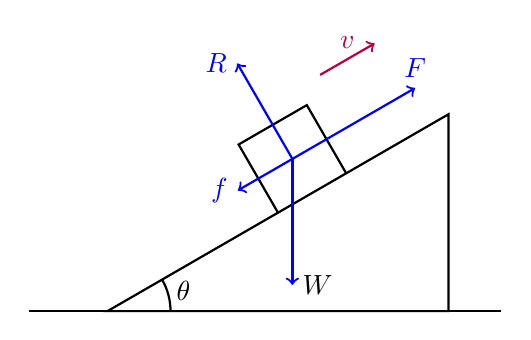
\begin{tikzpicture}[scale=1]
	\draw[thick] (0,0) -- (30:5) -- ++(0,-2.5) -- cycle;
	\draw[thick] (0.8,0) arc(0:30:0.8);
	\node at (15:1) {$\theta$};
	\draw[thick] (30:2.5) -- ++(120:1) -- ++(30:1) -- ++(-60:1);
	\draw[thick] (-1,0) -- (5,0);
	\draw[thick,blue,->] (2.348,1.933) --++ (0,-1.6) node[right,black]{$W$};
	\draw[thick,blue,->] (30:3) ++ (120:0.5) --++ (120:1.4) node[left]{$R$};
	\draw[thick,blue,->] (30:3) ++ (120:0.5) --++ (30:1.8) node[above]{$F$};
	\draw[thick,blue,->] (30:3) ++ (120:0.5) --++ (210:0.8) node[left]{$f$};
	\draw[purple,thick,->] (2.7,3) --++ (30:0.8) node[midway,above]{$v$};
	%	\draw[thick,blue,->] (2.348,1.933) --++ (210:0.8) node[left]{$W_\parallelslant$};
	%	\draw[thick,blue,->] (2.348,1.933) --++ (-60:1.38564) node[right]{$W_\perp$};;
	%	\draw[dashed] (2.348,1.933) ++ (210:0.8) --++ (-60:1.38564) --++ (30:0.8) ;
	\end{tikzpicture}
	\vspace*{-16pt}
\end{wrapfigure}

the problem is about a mass $m$ placed on a plane inclined at angle $\theta$ to the horizontal

the mass could sit at rest on, slide down, or get pulled/pushed up the plane

motion of the mass could be affected by weight, friction, normal contact, or other forces

\cmt forces can be resolved in directions parallel and perpendicular to the slope

resolving along the slope leads to the equation of motion from which acceleration is found

\cmt it is almost inevitable to break weight into two components\footnote{We have already done that in Example \ref{ex:comp-of-W}.}

\titem component of weight parallel down the slope is: $W_\parallelslant = mg\sin\theta$

\titem component of weight perpendicular to slope is: $W_\perp = mg\cos\theta$

\begin{wrapfigure}{r}{0.4\textwidth}
	\centering
	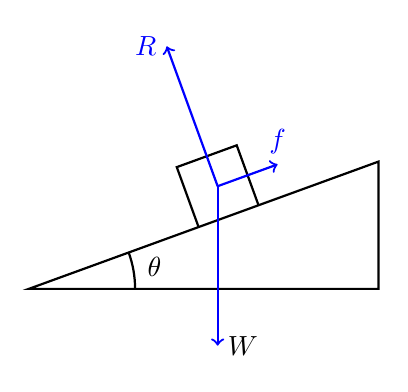
\begin{tikzpicture}[scale=1.35]
	\draw[thick] (0,0) -- (20:3.5) -- ++(0,-1.1971) -- cycle;
	\draw[thick] (1,0) arc(0:20:1);
	\node at (10:1.2) {$\theta$};
	\draw[thick] (20:1.7) -- ++(110:0.6) -- ++(20:0.6) -- ++(-70:0.6);
	\draw[thick,blue,->] (20:2) ++ (110:0.3) --++ (0,-1.5) node[right,black]{$W$};
	\draw[thick,blue,->] (20:2) ++ (110:0.3) --++ (110:1.4) node[left]{$R$};
	\draw[thick,blue,->] (20:2) ++ (110:0.3) --++ (20:0.6) node[above]{$f$};
	\end{tikzpicture}
	\vspace*{-16pt}
\end{wrapfigure}

\example{A block of mass $m$ stays at rest on an inclined plane. The plane makes an angle $\theta$ with the horizontal. Find the normal contact force $R$ and the frictional force $f$ acting on the block.}

\sol block in equilibrium, so $\fnet=0$ in any direction

parallel to slope: $f = W_\parallelslant \RA f=mg\sin\theta$

normal to slope: $R = W_\perp \RA R =mg\cos\theta$ \eoe


\begin{wrapfigure}{r}{0.4\textwidth}
	\centering
	\vspace*{-16pt}
	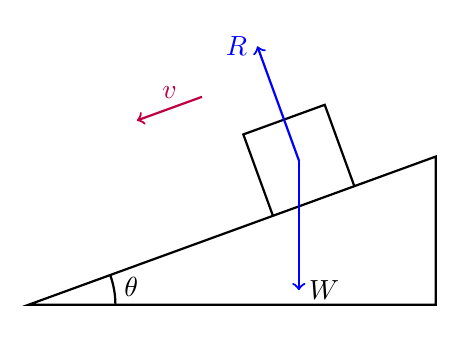
\begin{tikzpicture}[scale=1.1]
	\draw[thick] (0,0) -- (20:5) -- ++(0,-1.71) -- cycle;
	\draw[thick] (1,0) arc(0:20:1);
	\node at (10:1.2) {$\theta$};
	\draw[thick] (20:3) -- ++(110:1) -- ++(20:1) -- ++(-70:1);
	\draw[thick,blue,->] (20:3.5) ++ (110:0.5) --++ (0,-1.5) node[right,black]{$W$};
	\draw[thick,blue,->] (20:3.5) ++ (110:0.5) --++ (110:1.4) node[left]{$R$};
	\draw[purple,thick,->] (2,2.4) --++ (200:0.8) node[midway,above]{$v$};
	\end{tikzpicture}
	\vspace*{-16pt}
\end{wrapfigure}

\example{A block of mass $m$ slides down a \emph{smooth} slope. The angle of the slope to the horizontal is $\theta$. Find the acceleration of the block.}

\sol only force acting along the slope is component of weight down the slope, so:

{
	\centering
	
	$ \fnet = ma = mg\sin\theta \RA a = g\sin\theta $
	
}

as $\theta\to0$, $a\to0$, this shows if plane becomes horizontal, the block simply stays put

as $\theta\to90^\circ$, slope becomes vertical, block would undergo free fall, so naturally $a\to g$ \eoe 


\begin{wrapfigure}{r}{0.4\textwidth}
	\vspace*{25pt}
	\centering
	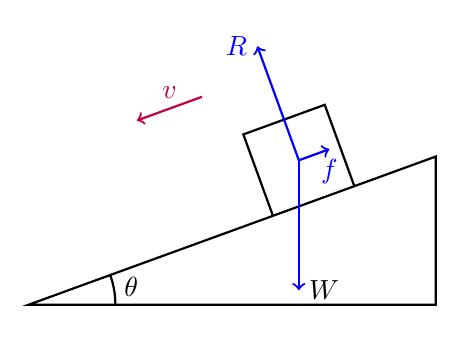
\begin{tikzpicture}[scale=1.1]
	\draw[thick] (0,0) -- (20:5) -- ++(0,-1.71) -- cycle;
	\draw[thick] (1,0) arc(0:20:1);
	\node at (10:1.2) {$\theta$};
	\draw[thick] (20:3) -- ++(110:1) -- ++(20:1) -- ++(-70:1);
	\draw[thick,blue,->] (20:3.5) ++ (110:0.5) --++ (0,-1.5) node[right,black]{$W$};
	\draw[thick,blue,->] (20:3.5) ++ (110:0.5) --++ (110:1.4) node[left]{$R$};
%	\draw[thick,blue,->] (20:3.5) ++ (110:0.5) --++ (20:1.8) node[above]{$F$};
	\draw[thick,blue,->] (20:3.5) ++ (110:0.5) --++ (20:0.375) node[below]{$f$};
	\draw[purple,thick,->] (2,2.4) --++ (200:0.8) node[midway,above]{$v$};
	%	\draw[thick,blue,->] (20:3.5) ++ (110:0.5) --++ (200:0.8) node[left]{$W_\parallelslant$};
	%	\draw[thick,blue,->] (20:3.5) ++ (110:0.5) --++ (-70:1.38564) node[right]{$W_\perp$};;
	%	\draw[dashed] (2.348,1.933) ++ (210:0.8) --++ (-60:1.38564) --++ (30:0.8) ;
	\end{tikzpicture}
%	\vspace*{-16pt}
\end{wrapfigure}

\newpage

\example{A block of mass 2.0 kg slides down a rough slope from rest. The slope is inclined at angle $\theta=20^\circ$ to the horizontal, and the block experiences a constant friction of 5.0 N. (a) What is the block's acceleration? (b) What is the distance travelled in 2.5 seconds?}

\sol resolving along slope:

{
	\centering
	
	$\fnet = mg\sin\theta - f = ma$
	
	\eqyskip $a = \frac{2.0 \times 9.81\times\sin20^\circ - 5.0}{2.0} \approx 0.855 \mpss $
	
}




distance travelled: $s = \cancelto{0}{ut} + \frac{1}{2}at^2 = \frac{1}{2}\times0.855\times2.5^2 \approx 2.67 \text{ m}$ \eoe


\begin{wrapfigure}{r}{0.4\textwidth}
%	\vspace*{16pt}
	\centering
	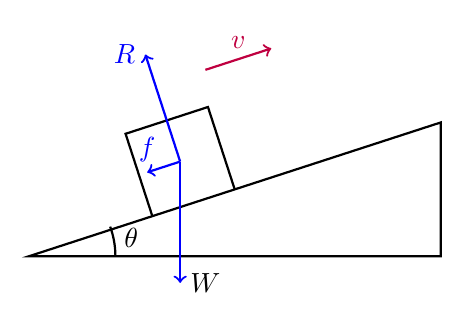
\begin{tikzpicture}[scale=1.1]
	\draw[thick] (0,0) -- (18:5) -- ++(0,-1.545) -- cycle;
	\draw[thick] (1,0) arc(0:20:1);
	\node at (10:1.2) {$\theta$};
	\draw[thick] (18:1.5) -- ++(108:1) -- ++(18:1) -- ++(-72:1);
	\draw[thick,blue,->] (18:2) ++ (108:0.5) --++ (0,-1.4) node[right,black]{$W$};
	\draw[thick,blue,->] (18:2) ++ (108:0.5) --++ (108:1.3) node[left]{$R$};
	%	\draw[thick,blue,->] (20:3.5) ++ (110:0.5) --++ (20:1.8) node[above]{$F$};
	\draw[thick,blue,->] (18:2) ++ (108:0.5) --++ (198:0.4) node[above]{$f$};
	\draw[purple,thick,<-] (2.8,2.4) --++ (198:0.8) node[midway,above]{$v$};
	%	\draw[thick,blue,->] (20:3.5) ++ (110:0.5) --++ (200:0.8) node[left]{$W_\parallelslant$};
	%	\draw[thick,blue,->] (20:3.5) ++ (110:0.5) --++ (-70:1.38564) node[right]{$W_\perp$};;
	%	\draw[dashed] (2.348,1.933) ++ (210:0.8) --++ (-60:1.38564) --++ (30:0.8) ;
	\end{tikzpicture}
	%	\vspace*{-16pt}
\end{wrapfigure}


\example{A block of mass 3.0 kg is travelling up an inclined slope at an initial speed of $2.8 \mps$. The slope makes an angle of $18^\circ$ with the horizontal. A constant friction of 7.5 N acts on the block. (a) What is the block's deceleration? (b) How far does the block travel along the slope before its speed decreases to zero? (c) Suggest whether the block could stay on the slope.}

\sol resolving along slope (take direction of initial velocity as positive direction): 

{
	\centering
	
	$\fnet = -mg\sin\theta - f = ma \RA a = \frac{-mg\sin\theta-f}{m} = \frac{-3.0\times9.81\times\sin18^\circ-7.5}{3.0} \approx - 5.53 \mpss$
	
	\eqyskip $v^2 - u^2 = 2as \RA s = \frac{v^2 - u^2}{2a} = \frac{0^2 - 2.8^2}{2\times(-5.5.3)} \approx 0.709 \text{ m}$ 
	
}

note that component of weight down the slope is: $W_\parallelslant = mg\sin\theta = 3.0\times9.81\times18^\circ \approx 9.1 \text{ N}$

$W_\parallelslant > f$, so friction is not enough to prevent block from sliding back down the slope \eoe






\subsection{many-body problems}

the problems we have been dealing with so far only involve one body

a mechanical system could consist of several objects that mutually interact

\cmt one can take each individual and look into the \textit{internal} forces between the objects of interest

for any force acting between objects \emph{within} system, there is an equal but opposite reaction force

\cmt the system can also be treated as a whole

we can analyse \textit{net external force} acting on entire system and work out combined acceleration



\newpage


\example{Two boxes $A$ and $B$ are placed on a smooth surface. They are accelerated together by a horizontal force $F$ as shown. Find the acceleration and the contact force between them.}

\begin{figure}[ht]
	\centering
	\begin{tikzpicture}[scale=0.8]
	\draw[thick, blue, ->] (-2,1) -- (0,1) node[midway, above]{$F$};
	\draw (0,0) rectangle (2,2);
	\draw (2,0) rectangle (4,2);
	\node at (1,1) {$A$};
	\node at (3,1) {$B$};
	\draw (-1,0) -- (5,0);
	\end{tikzpicture}	
\end{figure}

\sol free-body diagrams for $A$, $B$, and entire system are given below

\begin{figure}[ht]
	\centering
	\begin{minipage}{0.3\textwidth}
		\centering
		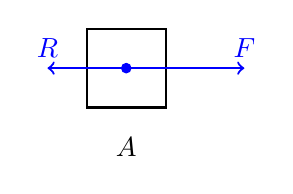
\begin{tikzpicture}
		\draw[thick] (-0.5,-0.5) rectangle (0.5,0.5);
		\draw[blue,fill] (0,0) circle(0.06);
		\draw[blue,thick,->] (0,0) -- (1.5,0) node[above]{$F$};
		\draw[blue,thick,->] (0,0) -- (-1,0) node[above]{$R$};
		\node at (0,-1) {$A$};
		\end{tikzpicture}
	\end{minipage}\hfil
	\begin{minipage}{0.3\textwidth}
		\centering
		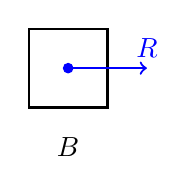
\begin{tikzpicture}
		\draw[thick] (-0.5,-0.5) rectangle (0.5,0.5);
		\draw[blue,fill] (0,0) circle(0.06);
		\draw[blue,thick,->] (0,0) -- (1,0) node[above]{$R$};
		\node at (0,-1) {$B$};
		\end{tikzpicture}
	\end{minipage}\hfil
	\begin{minipage}{0.3\textwidth}
		\centering
		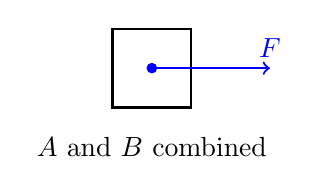
\begin{tikzpicture}
		\draw[thick] (-0.5,-0.5) rectangle (0.5,0.5);
		\draw[blue,fill] (0,0) circle(0.06);
		\draw[blue,thick,->] (0,0) -- (1.5,0) node[above]{$F$};
		\node at (0,-1) {$A$ and $B$ combined};
		\end{tikzpicture}
	\end{minipage}	
\end{figure}

\bxskip equations of motion can be written down for each free-body diagram and solved\footnote{In fact, only two of the three equations are independent. You can easily check that adding the equation for $A$ to that for $B$ would produce the equation for the system. To solve the two unknowns for this problem, any two of the three equations shall do the job. }
\begin{equation*}
\phantom{\Bigg\{\frac{frac{X}{X}}{frac{X}{X}}\Bigg\}^{\frac{X}{X}}}
\left\{\begin{array}{ll}
	\text{for $A$:} & F-R = M_A a \\
	\text{for $B$:} & R = M_B a \\
	\text{for system:} & F=(M_A+M_B)a
\end{array}\right.	\RA
\left\{\begin{array}{l}
a=\frac{F}{M_A+M_B} \phantom{\Bigg\{\frac{frac{X}{X}}{frac{X}{X}}\Bigg\}^{\frac{X}{X}}}\\
R= \frac{M_B}{M_A+M_B}F \phantom{\Bigg\{\frac{frac{X}{X}}{frac{X}{X}}\Bigg\}^{\frac{X}{X}}}
\end{array}\right. \teoe
\end{equation*}
	

\yskip\example{A vehicle of mass 1500 kg is towing a trailer of mass 500 kg by a light inextensible tow-bar. The engine of the vehicle exerts a driving force of 9600 N, and the tractor and the trailer experience resistances of 3600 N and 1800 N respectively. Find the acceleration of the vehicle and the tension in the tow-bar.}

\sol free-body diagrams for trailer, vehicle and entire system are given below

\begin{figure}[ht]
	\centering
	\begin{minipage}{0.15\textwidth}
		\centering
		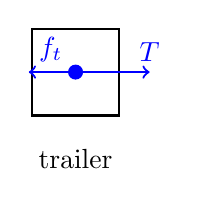
\begin{tikzpicture}[scale=1.1]
		\draw[thick] (-0.5,-0.5) rectangle (0.5,0.5);
		\draw[blue,fill] (0,0) circle(0.08);
		\draw[blue,thick,->] (0,0) -- (0.855,0) node[above]{$T$};
		\draw[blue,thick,->] (0,0) --++ (-0.54,0) node[above right]{$f_t$};
		\node at (0,-1) {trailer};
		\end{tikzpicture}
	\end{minipage}\hfil
	\begin{minipage}{0.38\textwidth}
		\centering
		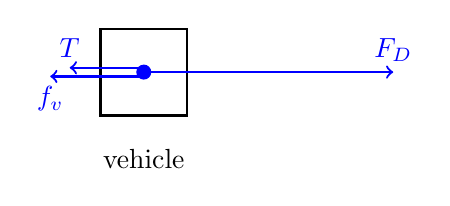
\begin{tikzpicture}[scale=1.1]
		\draw[thick] (-0.5,-0.5) rectangle (0.5,0.5);
		\draw[blue,fill] (0,0) circle(0.08);
		\draw[blue,thick,->] (0,0) -- (2.88,0) node[above]{$F_D$};
		\draw[blue,thick,->] (0,-0.05) --++ (-1.08,0) node[below]{$f_v$};
		\draw[blue,thick,->] (0,0.05) --++ (-0.855,0) node[above]{$T$};
		\node at (0,-1) {vehicle};
		\end{tikzpicture}
	\end{minipage}\hfil
	\begin{minipage}{0.38\textwidth}
		\centering
		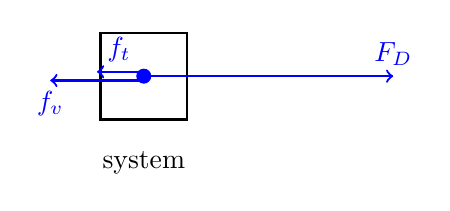
\begin{tikzpicture}[scale=1.1]
		\draw[thick] (-0.5,-0.5) rectangle (0.5,0.5);
		\draw[blue,fill] (0,0) circle(0.08);
		\draw[blue,thick,->] (0,0) -- (2.88,0) node[above]{$F_D$};
		\draw[blue,thick,->] (0,-0.05) --++ (-1.08,0) node[below]{$f_v$};
		\draw[blue,thick,->] (0,0.05) --++ (-0.54,0) node[above right]{$f_t$};
		\node at (0,-1) {system};
		\end{tikzpicture}
	\end{minipage}	
\end{figure}

\bxskip equations of motion can be written down for each free-body diagram:
\begin{equation*}
\left\{\begin{array}{ll}
\text{for trailer:} & T - f_t = M_t a \\
\text{for tractor:} & F_D - f_v - T = M_v a \\
\text{for system:} & F_D - f_v - f_t = (M_v + M_t)a
\end{array}\right.	\RA
\left\{\begin{array}{l}
T - 1800 = 500a \\
9600 - 3600 - T = 1500a \\
9600 - 3600 - 1800 = (1500 + 500)a
\end{array}\right.
\end{equation*}

\yskip solving simultaneous equations\footnote{Again, only two of the three equations are independent. You can freely choose your favourite two.}, we find
\begin{equation*}
a= 2.1 \mpss, \quad \text{and} \quad T=2850 \text{ N} \teoe
\end{equation*}
		
\subsubsection*{pulleys}

\begin{wrapfigure}{r}{0.21\textwidth}
	\vspace*{-24pt}
	\centering
	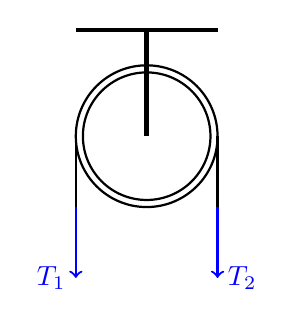
\begin{tikzpicture}[scale=0.9]
	\draw[thick] (0,0) circle(1) circle(0.9);
	\draw[thick] (1,0) --++ (0,-1);
	\draw[thick] (-1,0) --++ (0,-1);
	\draw[thick,blue,->] (1,-1) --++ (0,-1) node[right]{$T_2$};
	\draw[thick,blue,->] (-1,-1) --++ (0,-1) node[left]{$T_1$};
	\draw[ultra thick] (-1,1.5) -- (1,1.5) (0,1.5) -- (0,0);
	\end{tikzpicture}
	\vspace*{-16pt}
\end{wrapfigure}


a \emph{pulley} is basically a wheel that carries a string/rope/cable

in this section, we only consider pulleys whose axis of rotation is fixed

such pulleys can be used to change direction of tension in a taut string

we also assume pulleys to be \emph{ideal}: they have no mass and no friction

for an ideal pulley, tensions on both sides are equal: $T_1 = T_2$



\begin{wrapfigure}{r}{0.27\textwidth}
	\vspace{0pt}
	\centering
		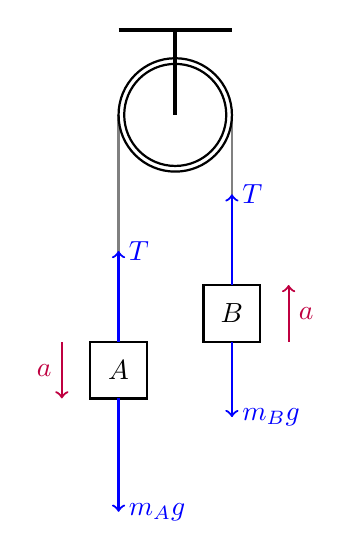
\begin{tikzpicture}[scale=0.72]
		\draw[thick,gray] (0, 0.5) -- (0,4.5);
		\draw[thick,gray] (2, 1.5) -- (2,4.5);
		\draw[thick]  (-0.5,-0.5) rectangle (0.5,0.5);
		\draw[thick]  (1.5,0.5) rectangle (2.5,1.5);
		\node at (0,0) {$A$};
		\node at (2,1) {$B$};
		\draw[thick] (1,4.5) circle(1) circle(0.9);
		\draw[ultra thick] (0,6) -- (2,6) (1,6) -- (1,4.5);
		\draw [blue, thick, ->] (0, 0.5) -- (0,2.1) node[right]{$T$};
		\draw [blue, thick, ->] (2, 1.5) -- (2,3.1) node[right]{$T$};
		\draw [blue, thick, ->] (0, -0.5) -- (0,-2.5) node[right]{$m_Ag$};
		\draw [blue, thick, ->] (2, 0.5) -- (2,-0.83) node[right]{$m_Bg$};
		\draw [purple, thick, <-] (-1, -0.5) -- (-1,0) node[left]{$a$} -- (-1,0.5);
		\draw [purple, thick, <-] (3, 1.5) -- (3,1) node[right]{$a$} -- (3,0.5);
		\end{tikzpicture}
	\vspace{-10pt}
\end{wrapfigure}

\example{Two blocks of mass $m_A$ and $m_B$ ($m_A>m_B$) are joined together by a light inextensible string. The string passes over a smooth pulley as shown. The two blocks are suddenly released from rest. Find the acceleration of each block and the tension in the string.}

\sol apply Newton's second law to each block:

{
	\centering
	
	$\left\{ \begin{array}{llll} \text{for $A$:} & m_Ag-T &=& m_Aa \\ \text{for $B$:} & T-m_Bg &=& m_Ba \end{array} \right.$
	
}

\vspace{0.4em} adding the two, one obtains equation of motion for whole system:

{
	\centering
	
	$ m_A g - m_B g = (m_A+m_B) a $
	
}

		
solving these equations, we find
\begin{equation*}
	a = \frac{m_A-m_B}{m_A+m_B}g \qquad T = \frac{2m_Am_Bg}{m_A+m_B} \teoe
\end{equation*}



\eqyskip\example{A mass $M=4.0 \text{ kg}$ is attached to a block of mass $m=2.0 \text{ kg}$ through	a light string which passes over a frictionless pulley as shown. When both masses are released, find the acceleration and the tension in the string.}

\begin{wrapfigure}{r}{0.45\textwidth}
	\centering
	\vspace*{-10pt}
	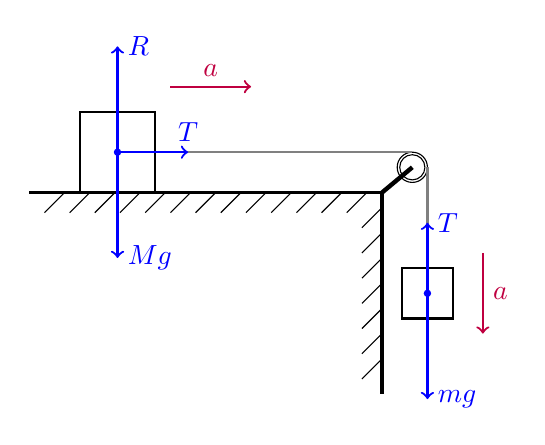
\begin{tikzpicture}[scale=0.64]
	\draw[thick] (-6,0) rectangle (-4.5,1.6);
	\draw[very thick] (-7,0) -- (0,0) -- (0,-4);
	\draw[thick] (0.4,-1.5) rectangle (1.4,-2.5);
	\draw[ultra thick] (0,0) -- (0.6,0.5) ;
	\draw (0.6,0.5) circle(0.3) circle(0.25);
	\draw[thick,gray] (-4.5,0.8) -- (0.6,0.8) (0.9,0.5) -- (0.9,-1.5);
	\draw[thick,blue,fill] (-5.25,0.8) circle(0.05);
	\draw[thick,blue,->] (-5.25,0.8) --++ (1.4,0) node[above]{$T$};
	\draw[thick,blue,->] (-5.25,0.8) --++ (0,-2.1) node[right]{$Mg$};
	\draw[thick,blue,->] (-5.25,0.8) --++ (0,2.1) node[right]{$R$};
	\draw[thick,blue,fill] (0.9,-2) circle(0.05);
	\draw[thick,blue,->] (0.9,-2) --++ (0,1.4) node[right]{$T$};
	\draw[thick,blue,->] (0.9,-2) --++ (0,-2.1) node[right]{$mg$};
	\foreach \x in {-0.3,-0.8,...,-6.3} \draw (\x,0) --++ (-0.4,-0.4);
	\foreach \y in {-0.3,-0.8,...,-3.3} \draw (0,\y) --++ (-0.4,-0.4);
	\draw[thick,purple,->] (2,-1.2) -- (2,-2.8) node[midway,right]{$a$};
	\draw[thick,purple,->] (-4.2,2.1) --++ (1.6,0) node[midway,above]{$a$};
	\end{tikzpicture}
\end{wrapfigure}

\sol apply Newton's second law to each mass:

{
	\centering
	
	$\left\{ \begin{array}{lcll} \text{for $M$:} & T &=& Ma \\ \text{for $m$:} & mg-T &=& ma \end{array} \right.$
	
}

\vspace{0.4em} adding the two equations, we have:

{
	\centering
	
	$ mg = (M+m) a $
	
}

so acceleration is:

{
	\centering
	
	$a = \frac{mg}{M+m} = \frac{2.0\times9.81}{4.0+2.0} = 3.27 \mpss$
	
}

tension in string: $T = Ma = 4.0 \times 3.27 \approx 13.1 \text{ N}$ \eoe



\ifthenelse{\includequestions=1}{
	
	
	
\subsection{end-of-chapter questions}

\subsubsection*{Newton's first law}

\question{A little girl tries to lift a luggage bag of mass 25 kg. She pulls upwards with a force of 150 N. The bag does not move. What is the normal reaction from the floor?}

\question{To push a trolley around in a supermarket with constant velocity, you need to exert a steady force. How does this fact agree with Newton's first law, which suggests that motion with constant velocity requires no force?}

\question{A worker is pulling a wagon of mass of 40 kg across a lawn at a constant velocity. He applies a force of 200 N at an angle of $15^\circ$ above the horizontal. (a) Draw a free-body diagram for the wagon. (b) Find the frictional force. (c) Find the normal contact force.}

\subsubsection*{Newton's second law}

\question{(a) Forces of 3.0 N and 4.0 N act at right angles upon a mass of 160 g. What is the acceleration produced? (b) If the angle between the two forces are allowed to vary, what is the maximum possible acceleration they produce on the same mass? (c) What about the minimum possible acceleration?}
	
\question{Explain why it becomes increasingly easier for an rocket to accelerate as it travels through space. (Hint: consider the fuel carried by the rocket.)}

\question{Many cars are equipped with airbags which can inflate quickly in case of a collision event. Using Newton's second law, suggest why airbags could protect the driver and the passenger in the car during a car crash.}

\question{A rocket of mass $30,000$ kg is launched vertically upwards at uniform acceleration of $1.6 \mpss$. What is the minimum thrust force required?}

\question{A fire-fighter of mass 85 kg slides down a vertical pole. He descends through a distance of 6.0 m in 2.0 seconds. (a) Find the average acceleration. (b) Find the average frictional force acting on the fire-fighter.}

\question{A trolley has mass $m$. A person needs to push the trolley with force $F$ to produce an acceleration of $a$, and with force $2F$ to produce an acceleration of $3a$. Find, in terms of $m$ and $a$, the constant resistive force opposing the trolley's motion.}

\question{A girl stands onto a bathroom scale and finds the reading is 35.0 \text{ kg}. She then takes the scale into a lift, what mass reading would she observe if the lift (a) is going down at a constant speed, (b) is accelerating downwards at $2.1 \mpss$?}

\question{A pirate finds a box of gold coins at the bottom of a lake. The box and its contents have a total mass of 40 kg. The pirate pulls on the box by means of a cable, so that the box is made to rise vertically through the water. Meanwhile, the flow of water creates a constant horizontal force on the box, and the upthrust on the box is known to be 150 N. At one instant, the pirate applies a force of 380 N at an angle of $25^\circ$ to the upward vertical, and the acceleration of the box is found to be $0.80 \mpss$. Assume all the forces acting are coplanar. (a) Draw a free-body diagram for the box. (b) Find the horizontal force due to water flow. (c) Find the drag force on the box.}



\subsubsection*{Newton's third law}

\question{A book placed on your desk experiences two forces: its weight and the support force. Identify the associated reaction forces.}

\question{A student deduces that a rocket travelling in space can never accelerate because the propelling force acting on the rocket is cancelled by an equal and opposite force. Explain why this statement is incorrect.}

\question{A U-shaped magnet lies on a top-pan balance and a mass reading of 180 g is registered. A current-carrying wire is then placed above the magnet. The wire experiences an additional force of 0.30 N that acts upwards. What is the mass reading on the balance?}

\subsubsection*{terminal velocity}

\question{A light ball and a heavy ball of the same size are released from a very high tower, state and explain whether they will reach the ground at the same time.}

\question{A stone is dropped from rest from a high tower. Air resistance is not negligible as the stone reaches terminal speed. Sketch two separate graphs to show the variation of its displacement and acceleration with time.}

\question{How does the terminal speed of a parachutist before opening the parachute compare to that after? Explain your reasons.}

\question{A ball is thrown horizontally from the top of a cliff. Effects of air resistance cannot be neglected. What happens to the horizontal and vertical components of the ball’s velocity?}

\question{A small sphere of mass 20.0 g is dropped from rest in a viscous liquid. When the sphere is moving at a speed of $v$, the viscous drag has a magnitude of $f = \alpha v^2$, where $\alpha=14 \text{ kg m}^{-1}$. (a) What is the sphere's acceleration at the instant when it is released? (b) What is the acceleration when it is moving at $5.0 \text{ cm s}^{-1}$? (c) What is the terminal velocity?}

\question{A stone is thrown with some initial velocity at an angle to the horizontal. Sketch on the same graph the path of the stone if (a) air resistance is negligible, (b) air resistance is significant.}

\subsubsection*{inclined slopes}

\question{A 3.0 kg mass is placed on an inclined plane and it does not move. Given that the normal contact force acting on it is 28.0 N. (a) Find the angle of the plane to the horizontal. (b) Find the frictional force acting on the mass.}

\question{A small mass slides down a frictionless slope with an acceleration of $2.8 \mpss$. Determine the angle that the slope makes with the horizontal.}

\question{A car of mass 1400 kg is moving up a slope at a constant velocity of $13.5\mps$. The slope makes an angle of $6.0^\circ$ to the horizontal. Total resistive force of 650 N acts on the car. What is the driving force required to push the car up the slope?}

\question{A shopping trolley somehow loses control and runs down a straight slope from rest. The slope makes an angle of $3.0^\circ$ to the horizontal. The resistive force acting on the trolley is a constant 15 N. The trolley and its contents have a total mass of 40 kg. (a) Find the acceleration of the trolley. (b) Determine the time for the trolley to travel a distance of 4.0 m along the the slope. (c) Suggest why the slope in shopping malls are not made any steeper.}

\question{A heavy log of mass 240 kg is initially placed at a point $P$ at the bottom of a slope. A motor drags the log up the slope through a cable. The slope is inclined at an angle of $16^\circ$ to the horizontal. The motor provides a tension of 1200 N parallel to the slope. The friction that acts on the log is a constant 450 N. (a) Find the acceleration of the log. (b) Find the time taken to pull the log through a distance of 8.0 m to a point $Q$. (c) Find the velocity of the log at $Q$. (d) The cable breaks when the log reaches $Q$, find the distance moved beyond $Q$ until the log's speed becomes zero. (e) The log will then slide back down the slope. Find the time for the log to return to its starting position. (f) Sketch a $v$-$t$ graph for the log from the start at $P$ until it returns to $P$.}

\subsubsection*{many-body problems}

\question{Block $A$ of mass 5.0 kg is connected by means of a light string to block $B$ of mass 3.0 kg. The two blocks are placed on a horizontal table. A force of 30 N is applied to pull on block $A$. Given that the friction on each block is 30\% of its own weight. (a) Find the acceleration of the blocks. (b) Find the tension in the string.}

\begin{wrapfigure}{r}{0.45\textwidth}
	\centering
	\vspace*{2pt}
	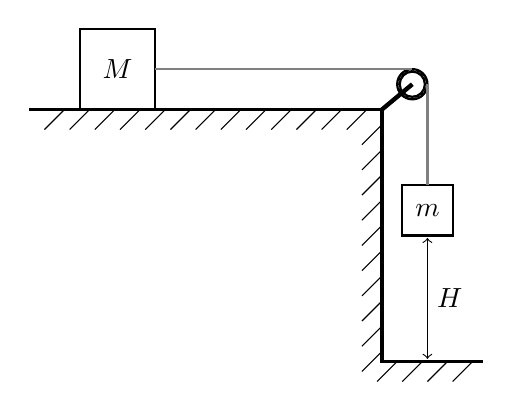
\begin{tikzpicture}[scale=0.64]
	\draw[thick] (-6,0) rectangle (-4.5,1.6);
	\node at (-5.25, 0.8) {$M$};
	\draw[very thick] (-7,0) -- (0,0) -- (0,-5) -- (2,-5);
	\draw[thick] (0.4,-1.5) rectangle (1.4,-2.5);
	\node at (0.9, -2) {$m$};
	\draw[ultra thick] (0,0) -- (0.6,0.5) ;
	\draw[thick] (0.6,0.5) circle(0.3) circle(0.25);
	\draw[thick,gray] (-4.5,0.8) -- (0.6,0.8) (0.9,0.5) -- (0.9,-1.5);
	\foreach \x in {-0.3,-0.8,...,-6.3} \draw (\x,0) --++ (-0.4,-0.4);
	\foreach \x in {0.3,0.8,...,1.8} \draw (\x,-5) --++ (-0.4,-0.4);
	\foreach \y in {-0.3,-0.8,...,-4.8} \draw (0,\y) --++ (-0.4,-0.4);
	\draw [<->] (0.9,0.05-5) -- (0.9,-0.05-2.5) node[midway,right]{$H$};
	\end{tikzpicture}
\end{wrapfigure}

\question{A box of mass $M=3.6 \text{ kg}$ rests on a horizontal, rough surface. The box is connected to a block of mass $m=2.0 \text{ kg}$ through a light cord that passes over a frictionless pulley as shown. The box is released from rest. Given that the box experiences a frictional force of 12 N and the block is initially at a height of $H=0.80 m$ above the floor. (a) Find the acceleration of the block. (b) Determine the time taken for the block to hit the floor.}



}{}